\documentclass[a4paper,14pt]{extarticle}


\usepackage[utf8]{inputenc}
\usepackage[T2A]{fontenc}
\usepackage[english,russian]{babel}
\usepackage{ragged2e}
\usepackage[utf8]{inputenc}
\usepackage{hyperref}
\usepackage{minted}
\setmintedinline{frame=lines, framesep=2mm, baselinestretch=1.5, bgcolor=LightGray, breaklines,fontsize=\scriptsize}
\setminted{frame=lines, framesep=2mm, baselinestretch=1.5, bgcolor=LightGray, breaklines,fontsize=\scriptsize}
\usepackage{xcolor}
\definecolor{LightGray}{gray}{0.9}
\usepackage{graphicx}
\usepackage[export]{adjustbox}
\usepackage[left=1cm,right=1cm, top=1cm,bottom=1cm,bindingoffset=0cm]{geometry}
\usepackage{fontspec}
\usepackage{ upgreek }
\usepackage[shortlabels]{enumitem}
\usepackage{adjustbox}
\usepackage{multirow}
\usepackage{amsmath}
\usepackage{amssymb}
\usepackage{pifont}
\usepackage{pgfplots}
\usepackage{longtable}
\usepackage{array}
\graphicspath{ {./images/} }
\makeatletter
\AddEnumerateCounter{\asbuk}{\russian@alph}{щ}
\makeatother
\setmonofont{Consolas}
\setmainfont{Times New Roman}

\newcommand\textbox[1]{
	\parbox{.45\textwidth}{#1}
} 

\newcommand{\specialcell}[2][c]{%
	\begin{tabular}[#1]{@{}c@{}}#2\end{tabular}}

\begin{document}
\pagenumbering{gobble}
\begin{center}
    \small{
        \textbf{МИНИCТЕРCТВО НАУКИ И ВЫCШЕГО ОБРАЗОВАНИЯ РОCCИЙCКОЙ ФЕДЕРАЦИИ}\\
        ФЕДЕРАЛЬНОЕ ГОCУДАРCТВЕННОЕ БЮДЖЕТНОЕ ОБРАЗОВАТЕЛЬНОЕ УЧРЕЖДЕНИЕ\\ВЫCШЕГО ОБРАЗОВАНИЯ \\
        \textbf{«БЕЛГОРОДCКИЙ ГОCУДАРCТВЕННЫЙ ТЕХНОЛОГИЧЕCКИЙ\\УНИВЕРCИТЕТ им. В. Г. ШУХОВА»\\ (БГТУ им. В.Г. Шухова)} \\
        \bigbreak
        
\includegraphics[width=70mm]{log}\\
        ИНСТИТУТ ИНФОРМАЦИОННЫХ ТЕХНОЛОГИЙ И УПРАВЛЯЮЩИХ СИСТЕМ\\}
\end{center}

\vfill
\begin{center}
    \large{
        \textbf{
            Лабораторная работа №5}}\\
    \normalsize{
        по дисциплине: Основы ИИ \\
        тема: «Решение оптимизационных задач эволюционно-генетическими алгоритмами»}
\end{center}
\vfill
\hfill\textbox{
    Выполнил: ст. группы ПВ-223\\Пахомов Владислав Андреевич
    \bigbreak
    Проверили: \\пр. Твердохлеб Виталий Викторович
}
\vfill\begin{center}
    Белгород 2025 г.
\end{center}
\newpage
\underline{\textbf{Цель работы: }}изучение особенностей генетических алгоритмов необходимых при решении оптимизационных задач.\\
\begin{center}
\textbf{Ход выполнения работы}
\end{center}


\includegraphics[width=140mm]{algorythm}\\

\href{https://github.com/IAmProgrammist/ai_basics/tree/lab3}{Ссылка на репозиторий}\\

Опыт №1: обычный сценарий\\
$p_{Mating} = 0.9$\\
$p_{Mutation} = 0.1$\\
Обычный сценарий. Алгоритм хорошо находит оптимальное решение и доходит до локального экстремума.\bigbreak

Опыт №2: кризис\\
$p_{Mating} = 0.1$\\
$p_{Mutation} = 0.1$\\
Слишком маленькая вероятность скрещивания приводит к маленькому разнообразию генов, и следовательно процесс поиска пути 
занимает гораздо большее время. И пусть симуляция кажется достаточно стабильной при таком подходе, на самом деле найденные
таким образом пути очень далеки от оптимальных.\bigbreak

Опыт №3: Чернобыль\\
$p_{Mating} = 0.9$\\
$p_{Mutation} = 0.9$\\
Слишком большой шанс мутаций слишком сильно портит рабочие гены, и не позволяет дойти до экстремума задачи. При таком способе решение, скорее, 
будет получено случайным перебором комбинаций, чем действительно генетическим алгоритмом.\bigbreak

Опыт №4: Сравнение времени работы с муравьиным алгоритмом\\
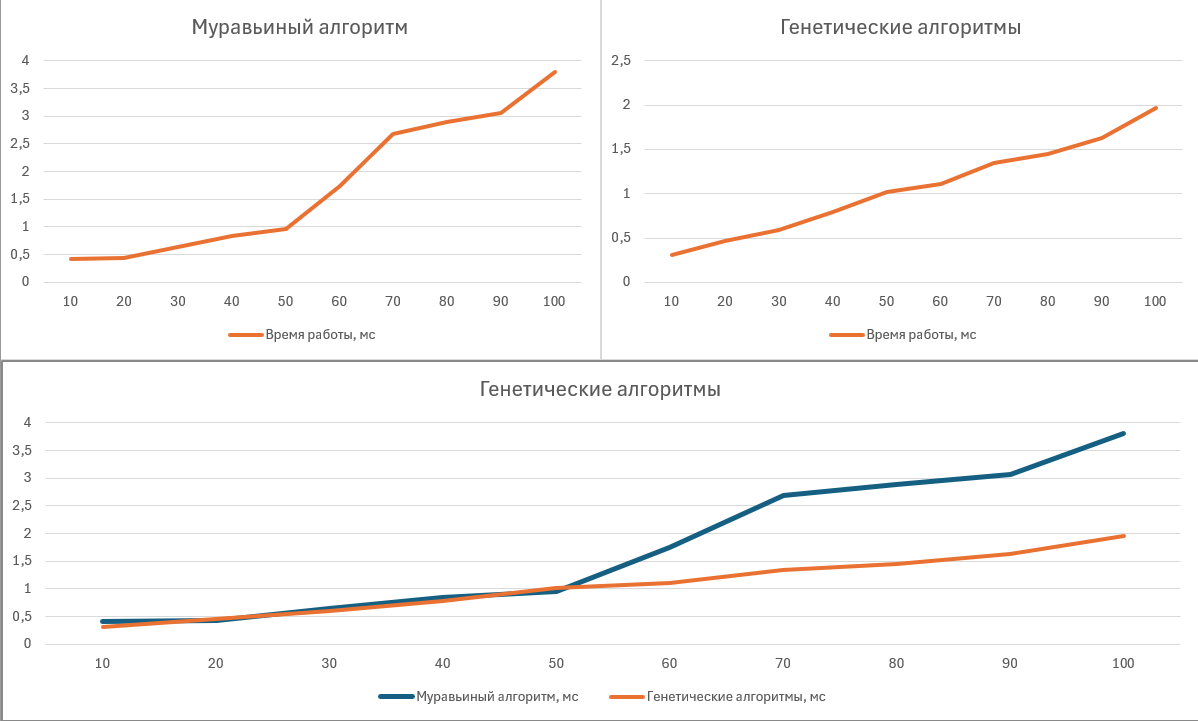
\includegraphics[width=140mm]{experiment}\\
Временная сложность муравьиного алгоритма в общем случае представляет собой $O(MN^2)$, где M - количество муравьёв, а 
N - количество городов. $N^2$ мы получаем из-за того, что каждый муравей должен в каждом городе обязательно просмотреть все доступные
города и выбрать лучший из них.

В то же время, генетический алгоритм при корректной реализации позволяет достигнуть сложности $O(MN)$. 

Предложенная реализация селекционирования приводила к сложности $O(M ^ 2)$, из-за поиска генов внутри массива, поэтому она была 
модифицирована. Мы также меняем порядок генов, но вместо этого мы меняем порядок генов в определённом диапазоне. Такой 
проход позволяет оптимизировать алгоритм до двух линейных проходов в $O(M)$. 

Алгоритм скрещивания, основанный на вероятностной модели, скорее всего приводил бы к $O(N log N)$ сложности, из-за того что 
нам бы каждый раз пришлось находить, на какой из генов упала "подкинутая монетка". Однако проход, основанный на обычном расчёте
количества генов, приводил к проблеме "полутора землекопов". Иначе говоря, сколько же генов нам нужно добавить, если их получилось
нецелое число. Для алгоритма скрещивания был выбран гибридный подход. Так, мы просчитываем целую часть количества генов, а уже на нецелую
часть количества генов мы "подбрасываем монетку". Такой подход позволит выполнить наиболее честное распределение а также
обеспечит сложность алгоритма $O(N)$.

\textbf{Вывод: } в ходе лабораторной работы изучили особенности генетических алгоритмов необходимых при решении оптимизационных задач.

\begin{minted}{Rust}
use core::f64;
use std::{error::Error, sync::{Arc, RwLock, RwLockReadGuard}};

use rand::Rng;

use crate::utils::ACOPaths;

// Функция-обёртка алгоритма скрещивания, позволяющая выбрать случайные индексы смешения генов
pub fn cross_parent(parent_a: &Vec<usize>, parent_b: &Vec<usize>) -> Result<Vec<usize>, Box<dyn Error>> {
    let mut rng = rand::rng();
    let gene_index_start = rng.random_range((0..parent_a.len()));
    let gene_index_end = rng.random_range((gene_index_start..parent_a.len()));

    return cross_within_mixup_range(parent_a, parent_b, gene_index_start, gene_index_end);
}

// Смешивает гены родителей и возвращает ребёнка
pub fn cross_within_mixup_range(parent_a: &Vec<usize>, parent_b: &Vec<usize>, mixup_low: usize, mixup_higher: usize) -> Result<Vec<usize>, Box<dyn Error>> {
    assert!(mixup_higher >= mixup_low);
    assert!(parent_a.len() == parent_b.len());

    let mut child = parent_b.clone();

    let mut parent_a_gene_index: usize = 0;
    let mut child_gene_index: usize = 0;

    while parent_a_gene_index < parent_a.len() && child_gene_index < child.len() {
        cross_find_next_gene_index(parent_a, mixup_low, mixup_higher, &mut parent_a_gene_index);
        cross_find_next_gene_index(&child, mixup_low, mixup_higher, &mut child_gene_index);

        if parent_a_gene_index >= parent_a.len() || child_gene_index >= child.len() {
            break;
        }

        child[child_gene_index] = parent_a[parent_a_gene_index];
        parent_a_gene_index += 1;
        child_gene_index += 1;
    }

    Ok(child)
}

pub fn cross_find_next_gene_index(specie_gens: &Vec<usize>, mixup_low: usize, mixup_higher: usize, gene_index: &mut usize) {
    while *gene_index < specie_gens.len() && (specie_gens[*gene_index] < mixup_low || specie_gens[*gene_index] > mixup_higher) {
        *gene_index += 1;
    }
}

pub fn cross(species: Vec<Vec<usize>>, mate_prob: f64) -> Vec<Vec<usize>> {
    // Выполняет скрещивание
    let mut cross_result: Vec<Vec<usize>> = Vec::new();
    let mut cross_result_idx = 0 as usize;

    // Выполним построение массива встреч
    let mut rng = rand::rng();
    let mating_arr: Vec<usize> = (0..(species.len() * 2)).map(|_| {
        rng.random_range(0..species.len())
    }).collect();

    for mate_idx in (0..mating_arr.len()).step_by(2) {
        // Если шанс встречи подходит, то выполняем скрещивание
        let mate_chance = rng.random_range((0.)..(1.));
        if mate_chance > mate_prob || mate_idx + 1 >= mating_arr.len() {
            continue;
        }

        let parent_a: Vec<usize> = species[mating_arr[mate_idx]].iter().map(|f| *f).collect();
        let parent_b: Vec<usize> = species[mating_arr[mate_idx + 1]].iter().map(|f| *f).collect();
        let child = cross_parent(&parent_a, &parent_b).unwrap();

        cross_result.push(child);
    }

    cross_result
} 

pub fn mutate(child: &Vec<usize>, mutation_prob: f64) -> Vec<usize> {
    let mut mutation_result = child.iter().map(|f| *f).collect();
    // Мутация - меняем случайный ген
    let mut rng = rand::rng();

    // Проверка на шанс мутации
    let mutation_chance = rng.random_range((0.)..(1.));
    if mutation_chance > mutation_prob {
        return mutation_result;
    }

    let gene_a_index = rng.random_range(0..mutation_result.len());
    let gene_b_index = rng.random_range(0..mutation_result.len());
    let tmp = child[gene_a_index];
    mutation_result[gene_a_index] = child[gene_b_index];
    mutation_result[gene_b_index] = tmp;
    return mutation_result;
}

// Создаём популяцию из случайных генов
pub fn create_population(genes_amount: usize, population_size: usize) -> Vec<Vec<usize>> {
    let mut rng = rand::rng();

    (0..population_size).map(|_| {
        let mut genes_array: Vec<usize> = (0..genes_amount).collect();

        for i in 0..genes_amount {
            let random_index = rng.random_range(0..genes_amount);
            let tmp = genes_array[i];
            genes_array[i] = genes_array[random_index];
            genes_array[random_index] = tmp;
        }

        genes_array
    }).collect()
}

// Выполняем селекцию
pub fn selection(species: &Vec<Vec<usize>>, paths: &RwLockReadGuard<'_, Arc<dyn ACOPaths>>, population_size: usize) -> Vec<Vec<usize>> {
    let mut rng = rand::rng();

    let mut selection_result = vec![vec![0 as usize; species[0].len()]; population_size];
    let mut roulette = vec![0.; species.len()];
    let mut roulette_sum = 0.;

    /* Сгенерировать рулетку */
    for (specie_index, specie) in species.iter().enumerate() {
        let mut path_len = 0.;
        for gene_index in 0..(specie.len() - 1) {
            path_len += paths.get_distance(specie[gene_index], specie[gene_index + 1]).unwrap();
        }
        path_len += paths.get_distance(*specie.last().unwrap(), specie[0]).unwrap();

        let specie_score = 1. / path_len;
        roulette[specie_index] = specie_score;
        roulette_sum += specie_score;
    }

    // На основе полученной рулетки добавляем виды
    let mut specie_current_idx: usize = 0;
    for i in 0..species.len() {
        if roulette[i] == -1. {
            continue;
        }
        let specie_amount_uneven = (roulette[i] / roulette_sum) * species.len() as f64;
        
        // Проблема полутора землекопов: что делать, если нам нужно добавить нецелое количество видов?
        // В этом случае мы гарантированно будем добавлять одного землекопа, а вот на половинку - 
        // будем подкидывать монетку.

        // Гибридный подход позволяет сохранить преимущества исключительно вероятностного
        // варианта алгоритма, а также скорость невероятностного варианта алгоритма. 
        // Также повышается "честность" выборки
        let specie_amount = specie_amount_uneven.trunc() as usize + 
        (if rng.random_range((0.)..(1.)) < specie_amount_uneven.fract() {1} else {0});
        for _ in 0..specie_amount {
            if specie_current_idx >= selection_result.len() {
                println!("Warning! A specie overflow");
                break;
            }

            selection_result[specie_current_idx] = species[i].iter().map(|it| *it).collect();
            specie_current_idx += 1;
        }
    }

    while specie_current_idx < population_size {
        selection_result[specie_current_idx] = selection_result[specie_current_idx - 1].iter().map(|it| *it).collect();
        specie_current_idx += 1;
    }

    selection_result
}


pub struct NextGenerationResult {
    pub species: Vec<Vec<usize>>,
    pub best_len: f64,
    pub best_genes: Vec<usize> 
}

// На основе полученного массива путей сгенерировать следующую популяцию а также возвращает индекс с
pub fn next_generation(species: &Vec<Vec<usize>>, paths: & mut Arc<dyn ACOPaths>, mate_prob: f64, mutation_prob: f64, population_size: usize) -> NextGenerationResult {
    let mut child_generation = Vec::new();
    let mut best_len = f64::INFINITY;
    let mut best_genes: Vec<usize> = vec![0; 0];
    
    {
        let field = Arc::new(RwLock::new(paths.clone()));
        let read_field = Arc::clone(&field);
        
        // Шаг 1: выполняем селекцию среди родительских генов
        let parent_generation = selection(species, &read_field.read().unwrap(), population_size);

        // Шаг 2: скрещиваем между собой родителей
        child_generation = cross(parent_generation, mate_prob);

        
        for i in 0..child_generation.len() {
            // Шаг 3: заставляем детей мутировать
            let child_mutate = mutate(&child_generation[i], mutation_prob);
            child_generation[i] = child_mutate;
        }

        // Теперь находим лучшую длину и набор генов
        for specie in child_generation.iter() {
            let mut path_len = 0.;
            for gene_index in 0..(specie.len() - 1) {
                path_len += paths.get_distance(specie[gene_index], specie[gene_index + 1]).unwrap_or(0.);
            }
            path_len += paths.get_distance(*specie.last().unwrap(), specie[0]).unwrap_or(0.);
            
            if path_len < best_len {
                best_len = path_len;
                best_genes = specie.iter().map(|f| *f).collect();
            }
        }
    }

    // Обновить феромон
    {
        let paths = Arc::get_mut(paths).ok_or("Failed").unwrap();
        for i in 0..paths.len() {
            for j in 0..paths.len() {
                paths.set_feromone_intensity(0., i, j);
            }
        }

        for gene_idx in 0..(best_genes.len() - 1) {
            paths.set_feromone_intensity(1., best_genes[gene_idx], best_genes[gene_idx + 1]);
        }

        paths.set_feromone_intensity(1., *best_genes.first().unwrap(), *best_genes.last().unwrap());
    }

    // Возвращаем поколение думеров
    return NextGenerationResult {species: child_generation, best_len, best_genes};
}
\end{minted}

\end{document}